% \section{Results overview and roadmap}

Plotting ideas for part 2:
\begin{itemize}
    \item The big important plot: Fuel level over time
    \item It would be interesting to see natural formation drift, and calculate delta-V requirements to compensate for this drift to estimate lifetime. This estimate could be used to validate results.
    \item Show the relative differences in applied perturbation acceleration from differential J2 and drag to explain drift rate
    \item Each subsystem should be validated in addition to showing the full fuel consumption over simulation duration:
    \begin{itemize}
        \item RW speed/torque step response
        \item Thruster force output as a function of fuel level (/tank pressure)
        \item MRP feedback controller tracking error and/or step response (would also be interesting to see a step response for different fuel levels)
        \item Decomposed net power and battery level (should also show the illumination factor in the same/adjacent plot and the FSW state)
    \end{itemize}
\end{itemize}

\section{Bsk Skf comparison}
State clearly that all differences are computed as Basilisk minus Skyfield.


\subsection{Overall Earth-relative Divergence}

\begin{figure}[H]
    \centering
    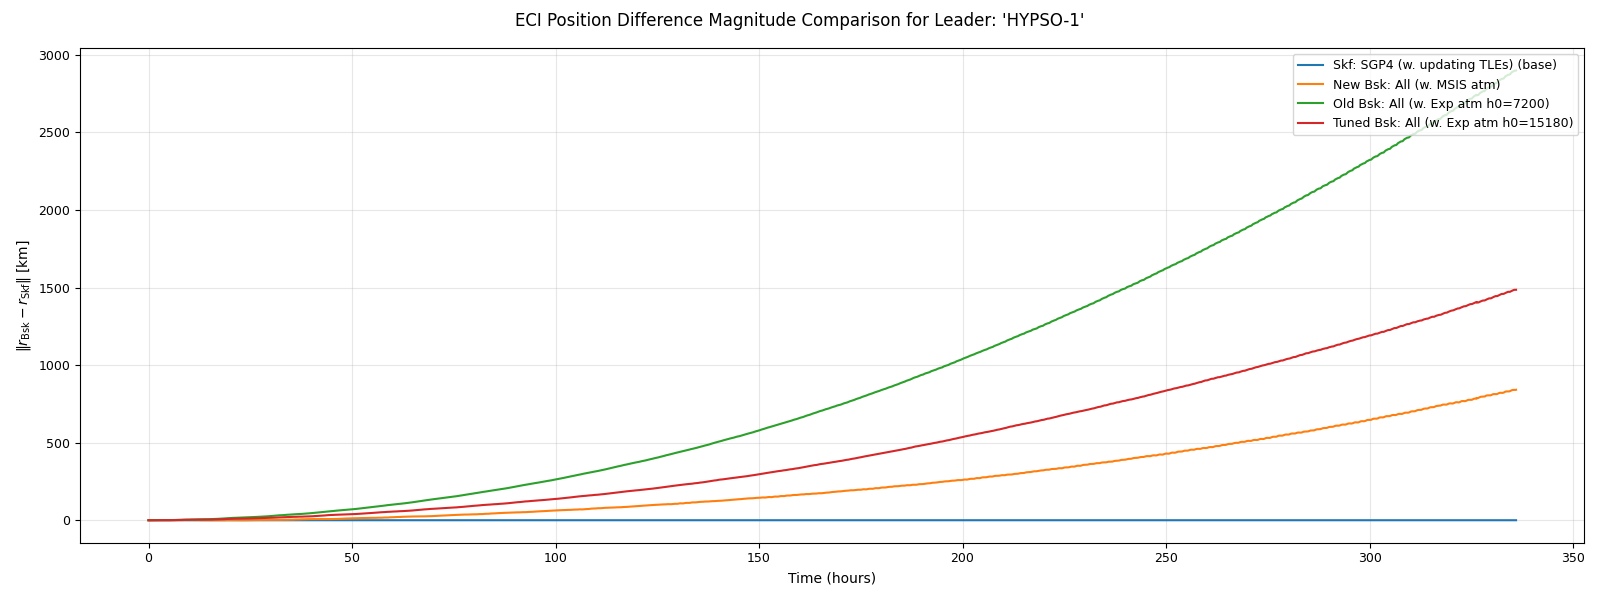
\includegraphics[width=0.6\textwidth]{Figures/05Results/bsk_skf_comparison/Ex1 - ECI pos difference magnitude.png}
    \caption{ECI position difference}
    \label{fig:1} 
\end{figure}

\begin{figure}[H]
    \centering
    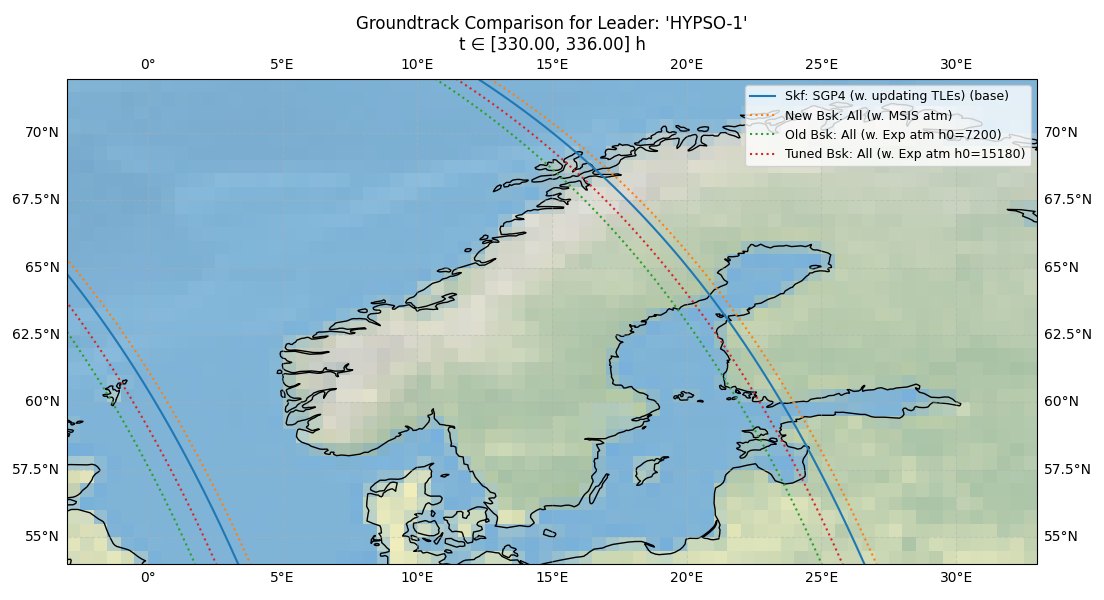
\includegraphics[width=0.6\textwidth]{Figures/05Results/bsk_skf_comparison/Ex1 - Groundtrack comparison.png}
    \caption{}
    \label{fig:2} 
\end{figure}



\subsection{Decomposition of Position Error in RTN Frame}

\begin{figure}[H]
    \centering
    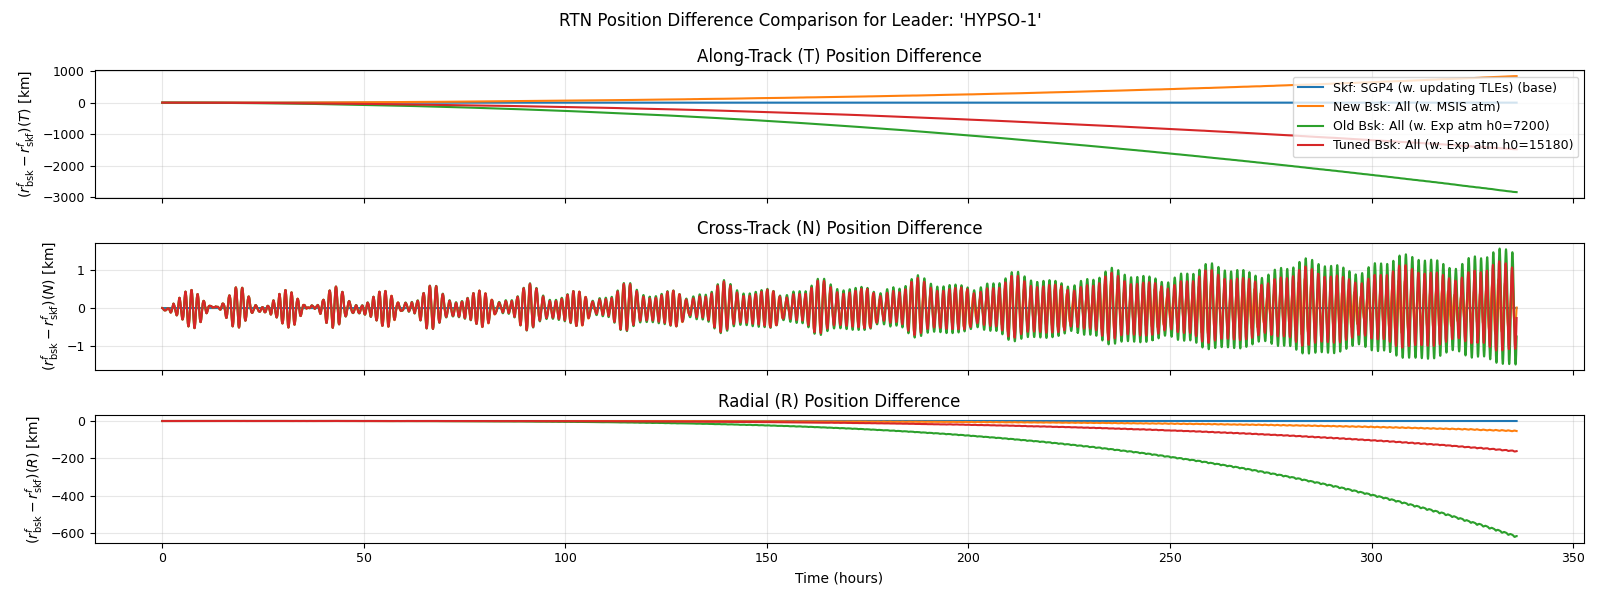
\includegraphics[width=0.6\textwidth]{Figures/05Results/bsk_skf_comparison/Ex1 - RTN pos difference.png}
    \caption{}
    \label{fig:3} 
\end{figure}



\subsection{Altitude Difference Comparison}

\begin{figure}[H]
    \centering
    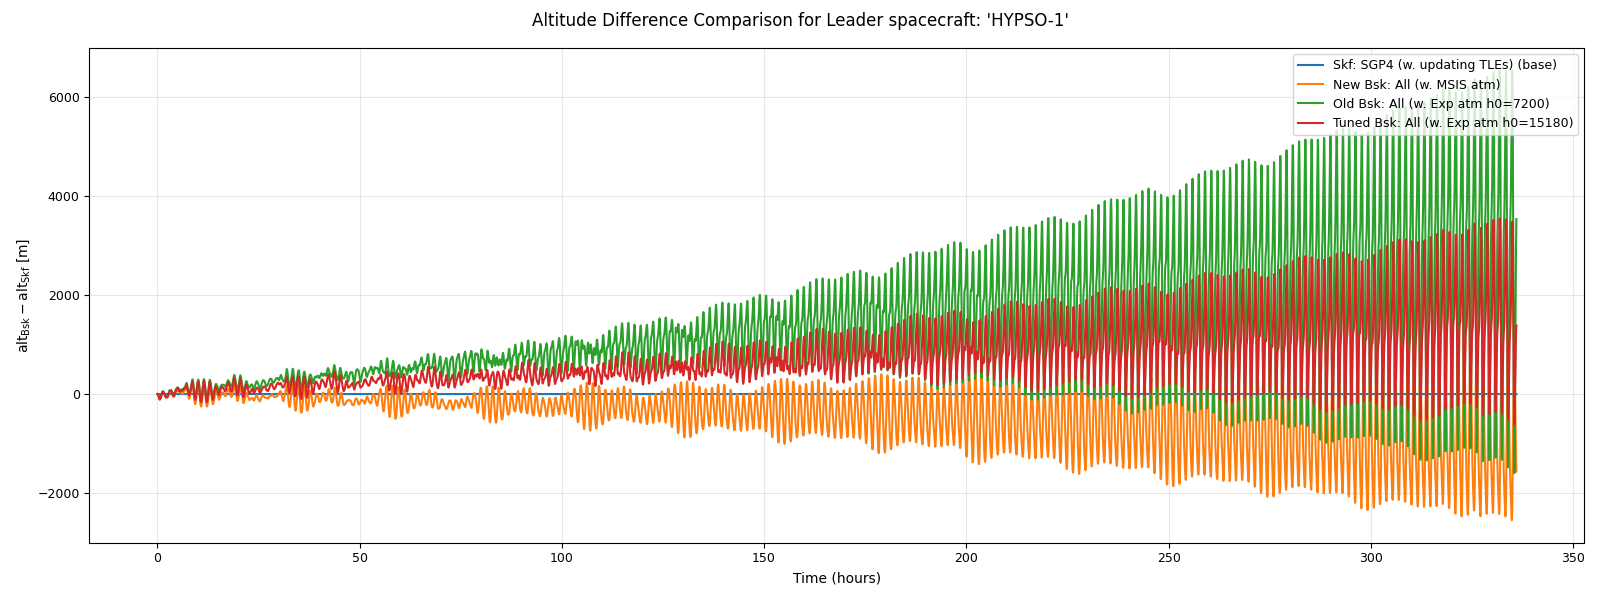
\includegraphics[width=0.6\textwidth]{Figures/05Results/bsk_skf_comparison/Ex1 - Altitude difference.png}
    \caption{}
    \label{fig:4} 
\end{figure}
\hl{I might try to remove some oscillations through data processing to highlight the trends and remove the altitude difference caused by different positions in the along-track and cross-track directions. Remove the }


\subsection{Orbital Element Drift}

\begin{figure}[H]
    \centering
    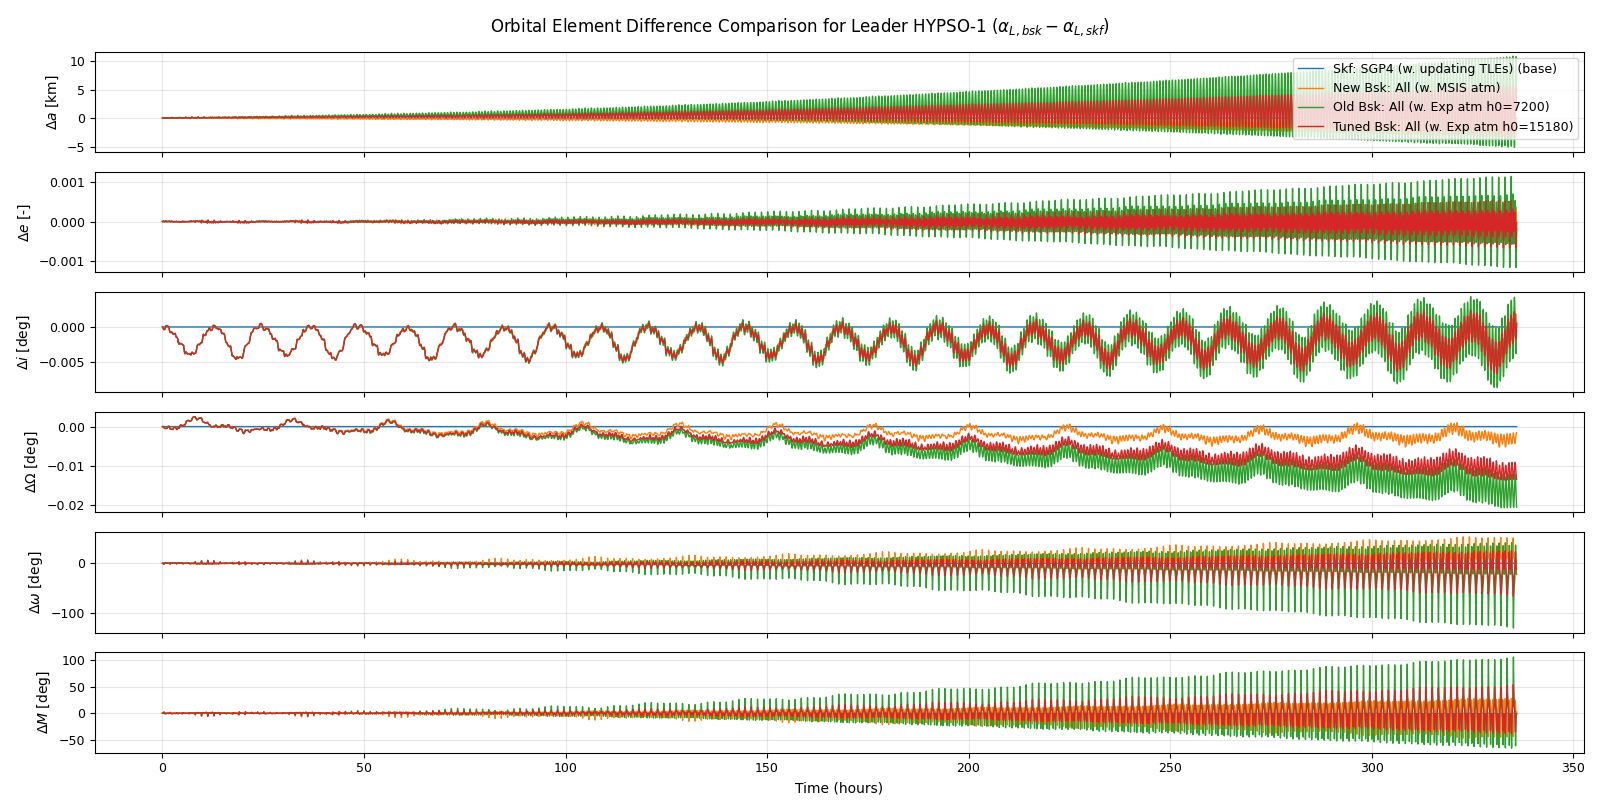
\includegraphics[width=0.6\textwidth]{Figures/05Results/bsk_skf_comparison/Ex1 - OE difference comparison.png}
    \caption{}
    \label{fig:5} 
\end{figure}

% \begin{figure}[H]
%     \centering
%     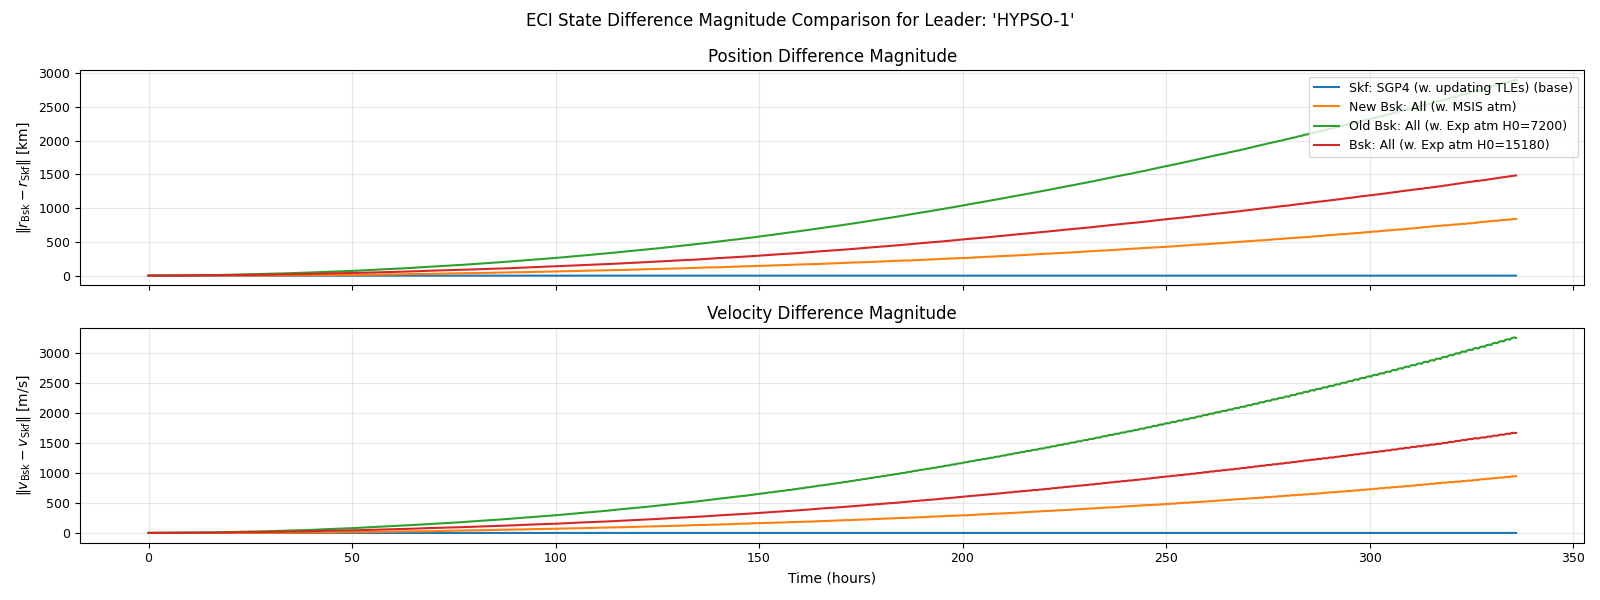
\includegraphics[width=0.6\textwidth]{Figures/05Results/bsk_skf_comparison/Ex1 - ECI pos-vel difference magnitude.png}
%     \caption{}
%     \label{fig:6} 
% \end{figure}


\subsection{Propagator Comparison Summary}

\begin{figure}[H]
    \centering
    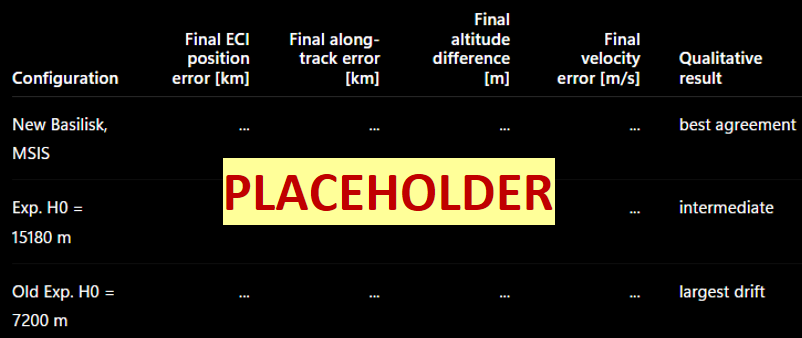
\includegraphics[width=0.6\textwidth]{Figures/05Results/bsk_skf_comparison/Bsk-Skf comparison summary table.png}
    \caption{Basilisk/Skyfield-SGP4 comparison summary}.
    \label{fig:bsk_skf_summary} 
\end{figure}








% ======================================================================================================================================= %
% ======================= G N S S - R    F O R M A T I O N    F L I G H T    S I M U L A T O R    R E S U L T S ======================= %
% ======================================================================================================================================= %


\section{Deployment Velocity Formation Acquisition Fuel Sensitivity}
\begin{comment}
This builds heavily on how "Formation Acquisition" is defined in the methodology

Data analysis that needs to be performed:

01. For each run, compute $t_{acq}$ and $m_{acq} = m_{fuel}(0) - m_{fuel}(t_{acq})$

02. For each run, compute the accumulated fuel consumption. This will enable other analyses and make comparisons simpler and more intuitive

Results that will be presented:


CORE PLOTS FOR THE DEPLOYMENT SENSITIVITY RESULT

1. Follower fuel consumption from all runs in one plot
    x-axis: time [h]
    y-axis: cumulative follower fuel consumed [g]
    one curve per deployment-speed case
    vertical marker at t_acq for each run, if acquired

2. Accumulated acquisition fuel consumption as a function of differential deployment speed
    x-axis: differential deployment speed magnitude [m/s]
    y-axis: acquisition fuel consumption [g]

3. Acquisition time as a function of differential deployment speed
    x-axis: differential deployment speed magnitude [m/s]
    y-axis: acquisition time [h]
4.1 RTN leader-follower relative position 3D trajectory for a selected set of runs
    RTN components in space
    choose subset of runs (0, 2, 4 diff speed)
4.2 RTN leader-follower relative positions decomposed for a selected set of runs
    choose subset of runs (0, 2, 4 diff speed)
    x-axis: time [h]
    y-axis: R, T, N components [m]
    horizontal lines for in-formation R, T, N upper/lower limit




SUPPORTING PLOTS FOR BURN Behavior 

5. Dual-bar plot showing acquisition accumulated thrust on-time and number of burns for each differential deployment speed
    x-axis: differential deployment speed magnitude [m/s]
    y-axis (left, corresponding to left vertical bar): acquisition accumulated thruster on-time / avg. thruster on-time
    y-axis (right, corresponding to right vertical bar): number of burns completed during acquisition


FEASIBILITY CHECKS

6. Operational mode timeline for all deployment cases / Another option is to show table with accumulated time spent in each mode for each run
    x-axis: time [h]
    y-axis: operational mode for each run
    show vertical lines for each run t_{acq}

7. Table summarizing some feasibility/accuracy metrics for each run:
    * The average attitude tracking error during burns [deg]
    * The accumulated time when burns were not possible (because of emergency mode)


SUMMARY TABLE

8. Show the following fields for every run:
    * Leader/follower deployment speed [m/s]
    * Differential speed [m/s]
    * Acquired?
    * Acquisition time [h]
    * Acquisition fuel [g]
    * Burns before acquisition
    * Avg. thruster on-time
    * Max RTN error [m]
    * Avg. attitude tracking error during burn
    * Min battery [%]



\begin{figure}[H]
    \centering
    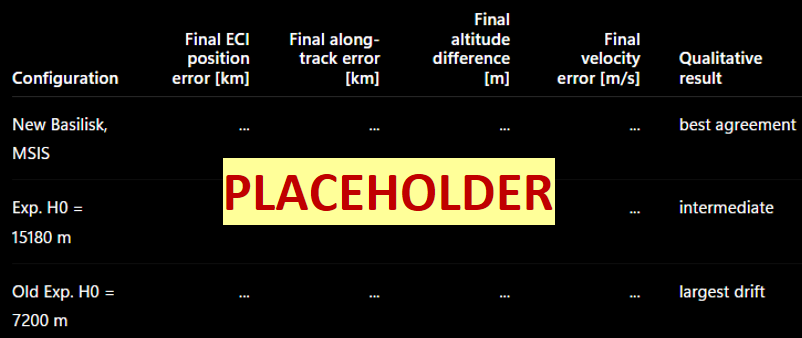
\includegraphics[width=0.6\textwidth]{Figures/05Results/bsk_skf_comparison/Bsk-Skf comparison summary table.png}
    \caption{Basilisk/Skyfield-SGP4 comparison summary}.
    \label{fig:bsk_skf_summary} 
\end{figure}



\end{comment}


\section{Steady-State Formation Maintenance Fuel Rate Estimation}
\begin{comment}


Supporting plot: 
Show the average pointing error during burns 


\end{comment}


\section{GNSS-R Formation Flight Lifetime Estimation}